\documentclass[12pt,letterpaper]{article}
\usepackage[utf8]{inputenc}
\usepackage{amsmath,amssymb,fullpage,graphicx}
\usepackage{subfigure}
\usepackage{amssymb}
\let\hat\widehat
\let\tilde\widetilde


%%\author{Nan Tang\\1662478}
	%% your name
%%\title{STAT 403 Spring 2018\\HW01}
	%% title of this document
\begin{document}
%%\maketitle
	%% make the title and author

\section*{Q4 }
For the one-sided test of the mean $\mu$ of a normal with known variance $\sigma^2$: \\
H0 : $\mu \leq 100 $ , H1 : $\mu > 100$. \\
The power curve for $\alpha = 0.05$ is $P_H1(\bar{X} \geq 100 + 1.645 * \frac{\sigma}{\sqrt{n}})$.

\subsection*{(a)}
\begin{verbatim}
library(ggplot2)
# for mu range from 100 to 110
mu.values <- seq(100, 110, 0.01)

# calculate power curve for given n, sigma, mu
# under alpha level 0.05
get.power.curve <- function(n1, sigma1, mu1) {
  k <- 100 + 1.645 * sigma1 / sqrt(n1)
  return(1 - pnorm(sqrt(n1) * (k - mu1) / sigma1))
}

# power curve when n = 25, sigma = 14
pc1 <- get.power.curve(25, 14, mu.values)

# power curve when n = 100, sigma = 14
pc2 <- get.power.curve(100, 14, mu.values)

# power curve when n = 25, sigma = 28
pc3 <- get.power.curve(25, 28, mu.values)

pc.combine <- data.frame(mu.values, pc1, pc2, pc3)

powercurve <- ggplot(data = pc.combine) +
  geom_line(aes(x=mu.values, y=pc1, linetype='n = 25, sigma = 14'), size=1) +
  geom_line(aes(x=mu.values, y=pc2, linetype='n = 100, sigma = 14'), size=1) +
  geom_line(aes(x=mu.values, y=pc3, linetype='n = 25, sigma = 28'), size=1) +
  labs(y="Power", 
       x="mu", 
       title="Power Curves (mu ranges from 100 - 110)",
       subtitle="Under the significance level of 0.05",
       linetype='n, sigma values'
       ) +
  scale_linetype_manual(values=c("solid", "dotted", "dotdash"))
theme_set(theme_bw())
plot(powercurve)
\end{verbatim}

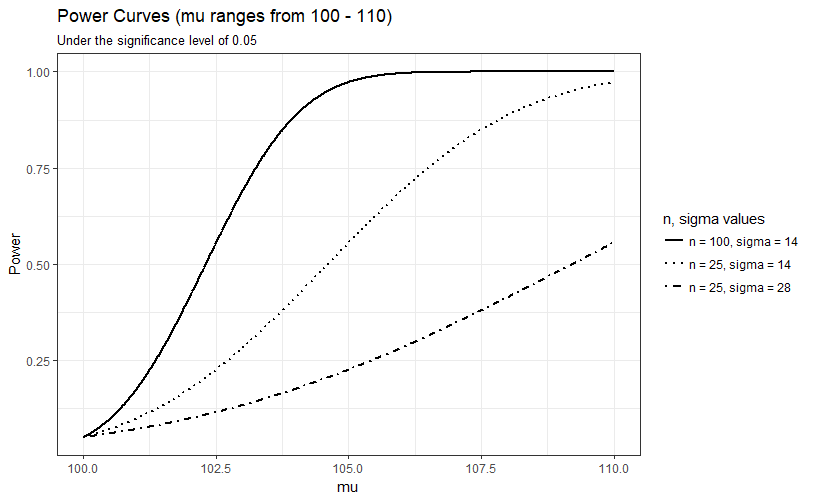
\includegraphics[width=170mm]{powercurve.png}
%%% do not touch anything below

\subsection*{(b)}
By comparing these three power curves with different sample size and population variance, we can see that as $\mu$ getting farther away from $\mu_0$, power of sample size 100 and population standard deviation 14 grows the fastest, and converges to $100\%$ power at $\mu = 106$. Power curve of sample size 25, population standard deviation 28 grows slowest, since big standard error makes test statistic harder to reject the null hypothesis, even if $\mu$ is much bigger than $\mu_0$. \\

\noindent  We may conclude that as $\mu$ getting farther away from $\mu_0$, the power of the test converges to $100\%$ faster in sample with large size $n$, and in population with relatively small variance $\sigma^2$. 

\end{document}
